\hypertarget{section-deployment-view}{%
\section{7 Deployment View}\label{section-deployment-view}}

\hypertarget{_infrastructure_level_1}{%
\subsection{Microsoft Azure Deployment}\label{_infrastructure_level_1}}

\begin{figure}[h]
  \centering
  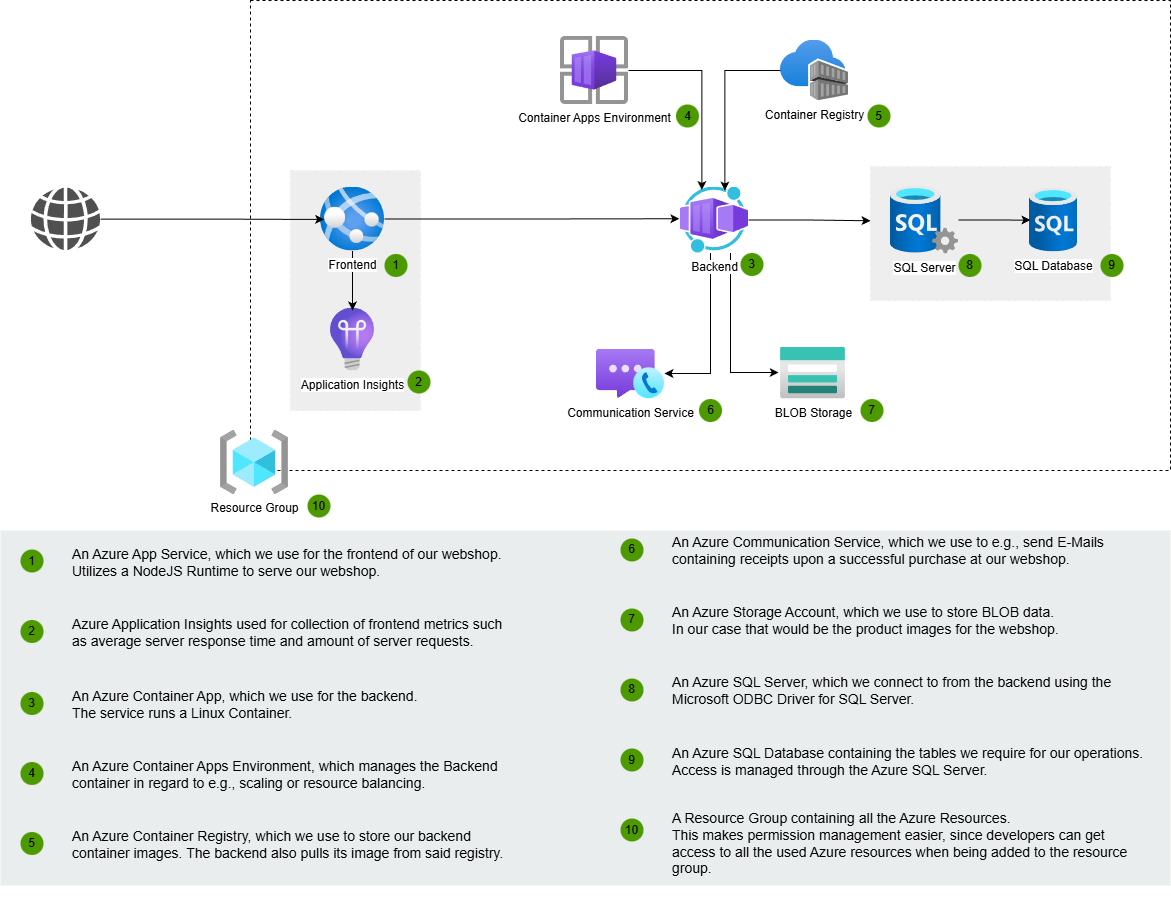
\includegraphics[width=\textwidth]{images/azure_deployment_view.png}
  \caption{Azure Infrastructure Diagram}
\end{figure}

\subsubsection{Motivation}
Instead of hosting the application locally on-premise, we instead opted for hosting it on the cloud.
This has multiple advantages such as not having to manage our own hardware as well as allowing more efficient resource utilization
by using a pay-as-you-go method of billing, rather than investing into our own hardware outright.

We chose to go forward with Microsoft Azure as our Cloud Service Provider, because they offer advanced features,
which we can make good use of, 
being reliable and easy to deploy with.

Now follow rationales for select services, where multiple Azure offerings could have been considered instead.

\begin{longtable}[]{@{}
  >{\raggedright\arraybackslash}p{(\columnwidth - 2\tabcolsep) * \real{0.3333}}
  >{\raggedright\arraybackslash}p{(\columnwidth - 2\tabcolsep) * \real{0.6667}}@{}}
\toprule
\begin{minipage}[b]{\linewidth}\raggedright
\textbf{Component}
\end{minipage} & \begin{minipage}[b]{\linewidth}\raggedright
\textbf{Rationale}
\end{minipage} \\
\midrule
\endhead
Frontend &
The frontend is served using NodeJS, therefore we deployed it using an Azure App Service,
since that is the most convenient way of deploying NodeJS applications on Azure. 
\\ \hline
Backend &
The python backend was designed as a Docker container in order to have e.g., rather simple horizontal scaling.
Therefore, it is suitable to use an Azure Container App to deploy the container into the cloud.
\\ \hline
Database &
As our database, we are utilizing the SaaS offering of Azure SQL Database, since it is generally more reliable
and more comfortable to work with, compared to hosting your own database with a PaaS offering.
Furthermore, we have personal preference toward managing relational databases, rather than non-relational databases.
Otherwise, we could have opted for non-relational database SaaS offering such as Azure Cosmos DB.
\\
\bottomrule
\end{longtable}

\subsubsection{Quality and/or Performance Features}
\begin{longtable}[]{@{}
  >{\raggedright\arraybackslash}p{(\columnwidth - 2\tabcolsep) * \real{0.3333}}
  >{\raggedright\arraybackslash}p{(\columnwidth - 2\tabcolsep) * \real{0.6667}}@{}}
\toprule
\begin{minipage}[b]{\linewidth}\raggedright
\textbf{Component}
\end{minipage} & \begin{minipage}[b]{\linewidth}\raggedright
\textbf{Quality and/or Performance Feature(s)}
\end{minipage} \\
\midrule
\endhead
Frontend &
The Azure App Service features 99.95\% guaranteed uptime as per the service-level agreement (SLA),
which is crucial for fulfilling our requirement of having high availability. 
\\ \hline
Backend &
The Azure Container App features the ability of creating replicas, allowing for horizontal scaling,
which can even be scaled automatically based on e.g., amount of concurrent incoming requests or CPU usage,
allowing for greater performance.
\\ \hline
Database &
The Azure SQL Database SaaS offering provides 99.99\% availability as per the service-level agreement.
This option allows for seamless upgrades to more premium service tiers, 
allowing for even availability guarantees exceeding 99.99\%.
Furthermore, more premium service tiers allow for using features, such as geo-redundant backup storage,
which replicates additional backups to a physical location hundreds of miles away from the primary region,
making it even more unlikely to lose significant amounts of data, even in catastrophic cases.
\\ \hline
BLOB Storage &
With Azure Storage Accounts, which we use for the blob storage, we have a 99.9\% availability as per the service-level agreement.
More premium options allow for going as high as 99.99\% availability.
\\ \hline
Azure Communication Services &
Azure Communication Services have an availability of 99.9\% guaranteed availability as per the service-level agreement,
making it so that our mailing service is highly available.
\\
\bottomrule
\end{longtable}

\subsubsection{Mapping}
Now follows a mapping of components in the building block view to components in the deployment view:

\subsubsection{Quality and/or Performance Features}
\begin{longtable}[]{@{}
  >{\raggedright\arraybackslash}p{(\columnwidth - 2\tabcolsep) * \real{0.3333}}
  >{\raggedright\arraybackslash}p{(\columnwidth - 2\tabcolsep) * \real{0.6667}}@{}}
\toprule
\begin{minipage}[b]{\linewidth}\raggedright
\textbf{Component in Building Block View}
\end{minipage} & \begin{minipage}[b]{\linewidth}\raggedright
\textbf{Component in Deployment View}
\end{minipage} \\
\midrule
\endhead
Frontend & 
\begin{itemize}
  \item App Service
  \item Application Insights
\end{itemize} \\ \hline
Backend & 
\begin{itemize}
  \item Container App
  \item Container Apps Environment
  \item Container Registry
\end{itemize} \\ \hline
E-Mail Service &
\begin{itemize}
  \item Communication Service
\end{itemize} \\ \hline
Database &
\begin{itemize}
  \item SQL Server
  \item SQL Database
\end{itemize} \\ \hline
\bottomrule
Image Storage &
\begin{itemize}
  \item Storage Account
\end{itemize} \\
\bottomrule
\end{longtable}